\begin{figure}[t]
  \centering
  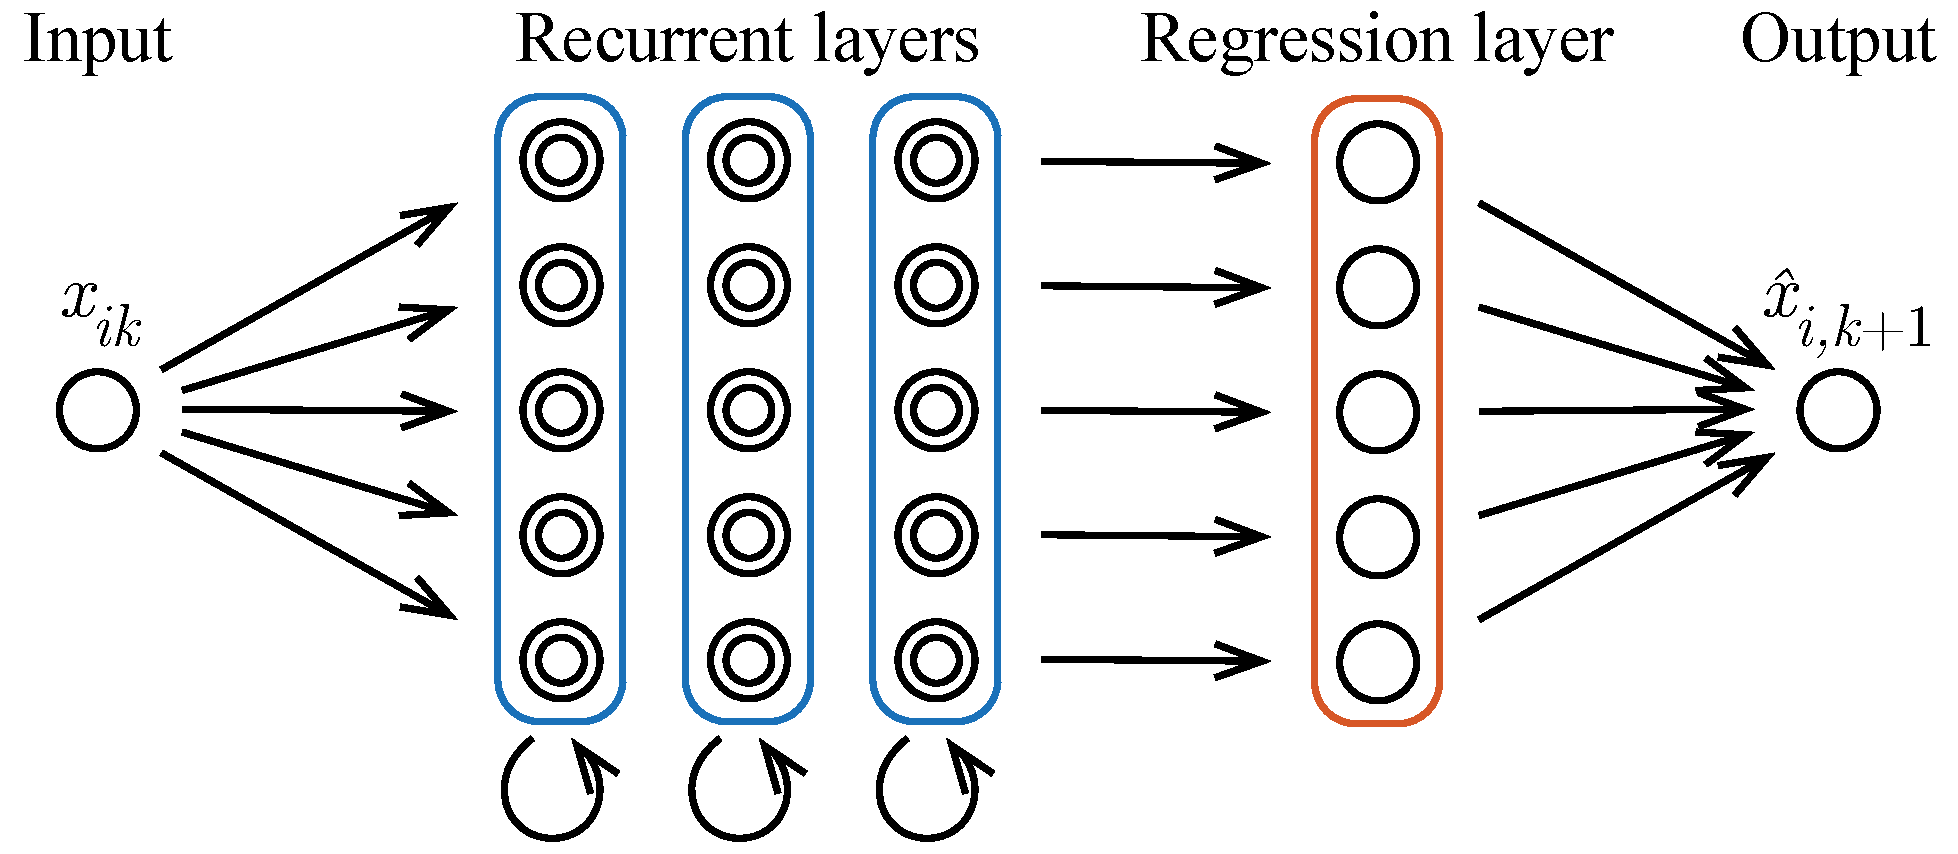
\includegraphics[width=1.0\columnwidth]{include/assets/figures/model.pdf}
  \caption{A schematic representation of our predictive model.}
  \vspace{-1.5em}
  \flab{model}
\end{figure}

As mentioned in \sref{introduction} and \sref{problem}, our goal is to assess
the applicability of the latest advancements in the development of neural
networks \cite{goodfellow2016} to modeling and prediction of fine-grained
resource-usage data. A neural network is a rather broad term: one network can be
nothing like another. Since the data that we study are inherently sequential, it
is natural to found our model on the basis of recurrent neural networks
\cite{goodfellow2016}, which are specifically designed for such cases as ours.

A schematic representation of our model can be seen in \fref{model}; many of the
actual connections between the model's parts are simplified or not shown at all
in order to make the figure legible. Let us now we describe each part in detail.

\subsection{Input and Output}
The input to the model is a single $d$-dimensional data point, which is
illustrated on the left-hand side of \fref{model}. Similarly, the output is a
single $d$-dimensional data point, which is depicted on the right-hand side of
\fref{model}. The input $x_{ik}$ represents the value of the resource usage of
an individual task at time step $k$, and the output $\hat{x}_{i,k + 1}$ is the
value at time step $k + 1$.

In order to have a long-range prediction (multiple steps ahead), we use
refeeding: the predicted value $\hat{x}_{i,k + 1}$ is fed into the model as if
it was the actual resource usage $x_{i,k + 1}$ at step $k + 1$, which is not
yet known at time step $k$. The process continues until all the desired $h$
future values are estimated.

\subsection{Recurrent Layers}
The core of the model is a recurrent neural network, which is depicted by a
group of three blue blobs in \fref{model}. Each such blob represents a single
recurrent layer, which we shall also refer to as a cell, and the network can be
made as many layers deep as needed. Each cell is composed of a number of units.

In addition, each cell is wrapped into a dropout layer \cite{zaremba2014}, which
gives control over the regularization of the model.

\subsection{Fully Connected Layer}
She sells seashells on the seashore.
